\chapter{Pré-processamento de Dados}
\label{chap:preprocessamento_de_dados}

\section{Preparação dos Dados}
Para este estudo, os dados foram coletados em sessões experimentais com atletas profissionais de basquetebol feminino, submetidas a duas condições: estimulação transcraniana por corrente contínua de alta definição (HD-tDCS) catódica e uma condição de controle (sham). Neste capítulo, descrevemos os procedimentos adotados para organizar, sincronizar e preparar os sinais de eletroencefalografia (EEG) e eletrocardiografia (ECG) para análise.

\subsection{Organização Inicial dos Dados}
Os dados de EEG e ECG foram armazenados em arquivos separados, correspondentes a cada atleta e a cada condição experimental (\textit{pre\_sham}, \textit{post\_sham}, \textit{pre\_cathodic}, \textit{post\_cathodic}). Os sinais de EEG foram originalmente registrados a 1000 Hz, enquanto os sinais de ECG – obtidos a partir do EMG do músculo peitoral maior – foram registrados a 1111,11 Hz. Nesta etapa, os arquivos passaram por:
\begin{itemize}
    \item Identificação e associação a cada atleta e condição;
    \item Renomeação e normalização para garantir consistência;
    \item Verificação de integridade para evitar erros no processamento.
\end{itemize}

\subsection{Sincronização Temporal entre EEG e ECG}
Devido ao início não sincronizado das gravações, foi necessário alinhar os sinais de EEG e ECG temporalmente. Com base em marcadores do período baseline, os seguintes procedimentos foram realizados:
\begin{itemize}
    \item Extração dos tempos de início e fim do baseline para cada modalidade;
    \item Ajuste dos timestamps para que os sinais iniciassem simultaneamente.
    \item Remoção dos primeiros e últimos 15 segundos de cada gravação, a fim de minimizar artefatos de borda;
\end{itemize}

\subsection{Estruturação dos Dados}
Após a sincronização, os dados foram organizados para o processamento subsequente. Os sinais de EEG foram armazenados em formato FIF, preservando as informações dos canais e os metadados, enquanto os dados de ECG foram exportados em formato CSV.
\section{Pré-processamento dos Sinais}

Esta seção descreve os procedimentos aplicados para garantir a qualidade dos sinais, abrangendo etapas de filtragem, remoção de artefatos e segmentação, com foco especial no processamento dos dados de EEG.

\subsection{Pré-processamento do EEG}

O processamento dos dados de EEG compreende duas etapas principais: a preparação dos dados brutos e a limpeza de artefatos utilizando técnicas de decomposição.

\subsubsection{Filtragem, Reamostragem e Preparação dos Dados de EEG}
Para a preparação dos dados de EEG, foram realizadas as seguintes etapas:
\begin{itemize}
    \item \textbf{Aquisição e Carregamento:} Os dados brutos foram baixados do Google Drive e carregados utilizando a biblioteca MNE-Python a partir de arquivos exportados do software BrainVision (ou, alternativamente, em formato EEGLAB). Após o carregamento, os canais foram renomeados conforme uma convenção padronizada (por exemplo, Fp1, Fz, F3, etc.) e canais irrelevantes foram removidos. (Ver Figura~\ref{fig:exemplo_sinais_eeg})
    \item \textbf{Aplicação de Montage:} Aplicou-se o montage padrão \textit{standard\_1005} para assegurar a correta localização dos eletrodos, conforme ilustrado no diagrama do sistema 10-20. (Ver Figura~\ref{fig:sistema_10_20})
    \item \textbf{Definição do Período de Análise:} Com base nas informações extraídas dos arquivos de baseline, os dados foram recortados para excluir os primeiros e últimos 15 segundos da gravação, reduzindo artefatos de borda.
    \item \textbf{Filtragem:} Foi aplicado um filtro passa-banda entre 0,5 e 60 Hz para eliminar ruídos fora do intervalo de interesse, seguido de um filtro notch em 60 Hz para remover interferências da rede elétrica.
    \item \textbf{Reamostragem:} Para padronizar a taxa de amostragem e facilitar o alinhamento com outros sinais (como o ECG), os dados de EEG foram reamostrados para 500 Hz.
\end{itemize}

\begin{figure}[htb]
    \centering
    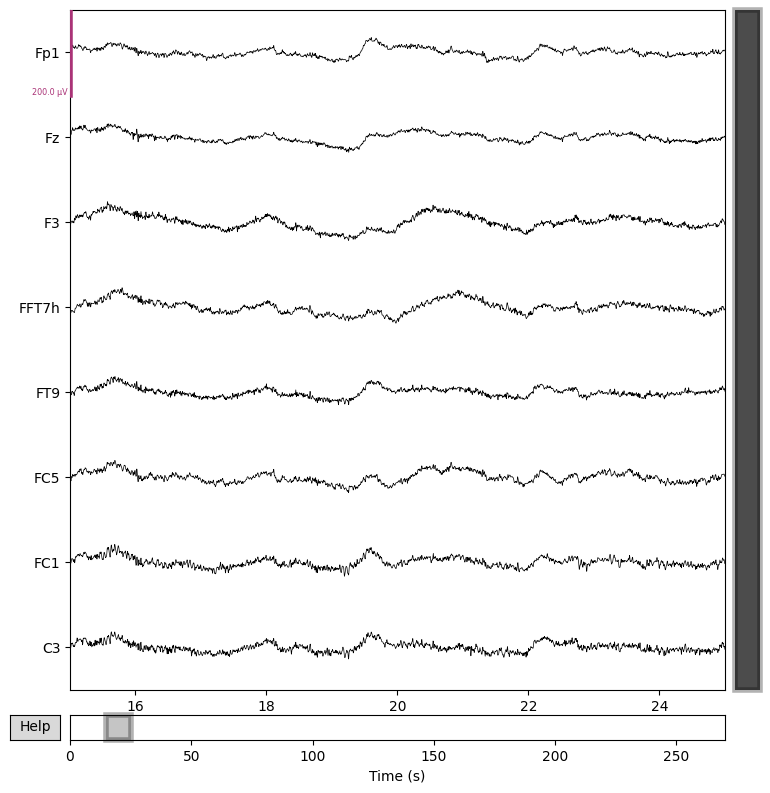
\includegraphics[width=0.8\textwidth]{figs/1_preprocessamento_eeg/2_exemplo_sinais_canais_eeg.png}
    \caption{Exemplo de sinais brutos de EEG, ilustrando a variação natural dos canais ao longo do tempo.}
    \label{fig:exemplo_sinais_eeg}
\end{figure}

\begin{figure}[htb]
    \centering
    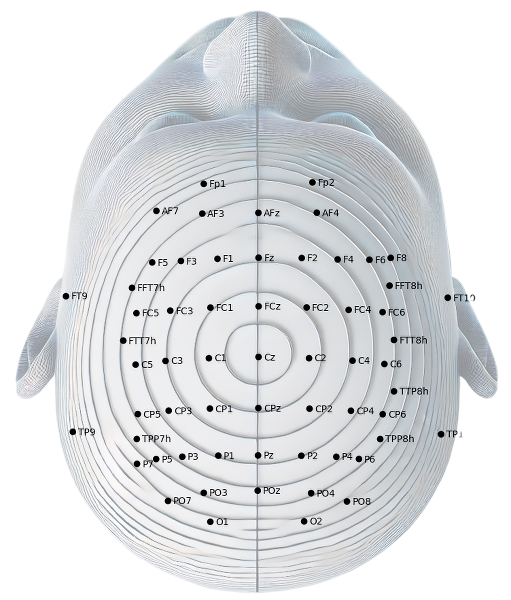
\includegraphics[width=0.8\textwidth]{figs/1_preprocessamento_eeg/1_sistema_10_20.png}
    \caption{Diagrama do sistema 10-20, demonstrando a localização padronizada dos eletrodos no couro cabeludo.}
    \label{fig:sistema_10_20}
\end{figure}

\subsubsection{Limpeza de Artefatos e Remoção de Componentes de Ruído (ICA)}
Para aprimorar a qualidade dos sinais de EEG, empregou-se a Análise de Componentes Independentes (ICA) seguindo os seguintes passos:
\begin{itemize}
    \item \textbf{Definição dos Componentes:} O número de componentes foi definido igual ao número de canais bons disponíveis (excluindo os canais previamente identificados como ruins por inspeção visual).
    \item \textbf{Aplicação do ICA:} Utilizou-se o método FastICA para decompor o sinal, preservando as informações essenciais para a análise de sincronicidade.
    \item \textbf{Estimativa de Parâmetros de Rejeição:} A biblioteca \textit{autoreject} foi empregada para determinar, por meio de épocas de duração fixa, os limites ideais para a rejeição de artefatos.
    \item \textbf{Identificação Automática de Artefatos:} Componentes associados a artefatos oculares (utilizando canais como Fp1 e Fp2) e à atividade cardíaca foram identificados automaticamente. Adicionalmente, uma análise baseada na curtose foi realizada para detectar componentes com alta amplitude, indicativos de artefatos.
    \item \textbf{Inspeção Visual e Seleção:} Foram gerados gráficos das propriedades dos componentes e uma visualização interativa (inclusive com animação GIF), permitindo a inspeção manual para a decisão de exclusão dos componentes indesejados. (Ver Figura~\ref{fig:componentes_pos_ICA})
    
    \item \textbf{Aplicação e Salvamento:} Após a definição dos componentes a serem removidos, o ICA foi aplicado para eliminar os artefatos identificados, gerando um sinal de EEG limpo, que foi salvo em formato FIF para futuras análises.
\end{itemize}

\begin{figure}[htb]
    \centering
    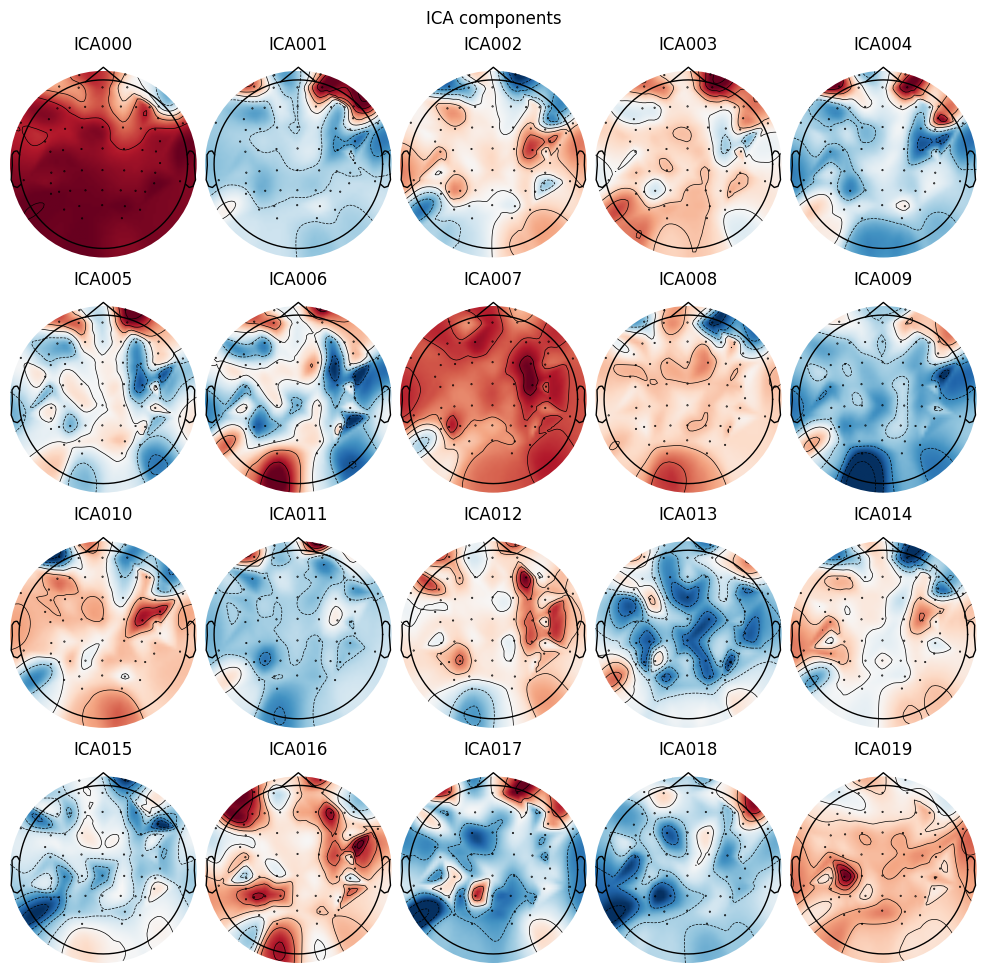
\includegraphics[width=0.8\textwidth]{figs/1_preprocessamento_eeg/3_exemplo_compomentes_pos_ICA.png}
    \caption{Exemplo de componentes obtidos após a aplicação do ICA, com mapas topográficos que evidenciam a distribuição espacial de cada componente.}
    \label{fig:componentes_pos_ICA}
\end{figure}

\begin{figure}[htb]
    \centering
    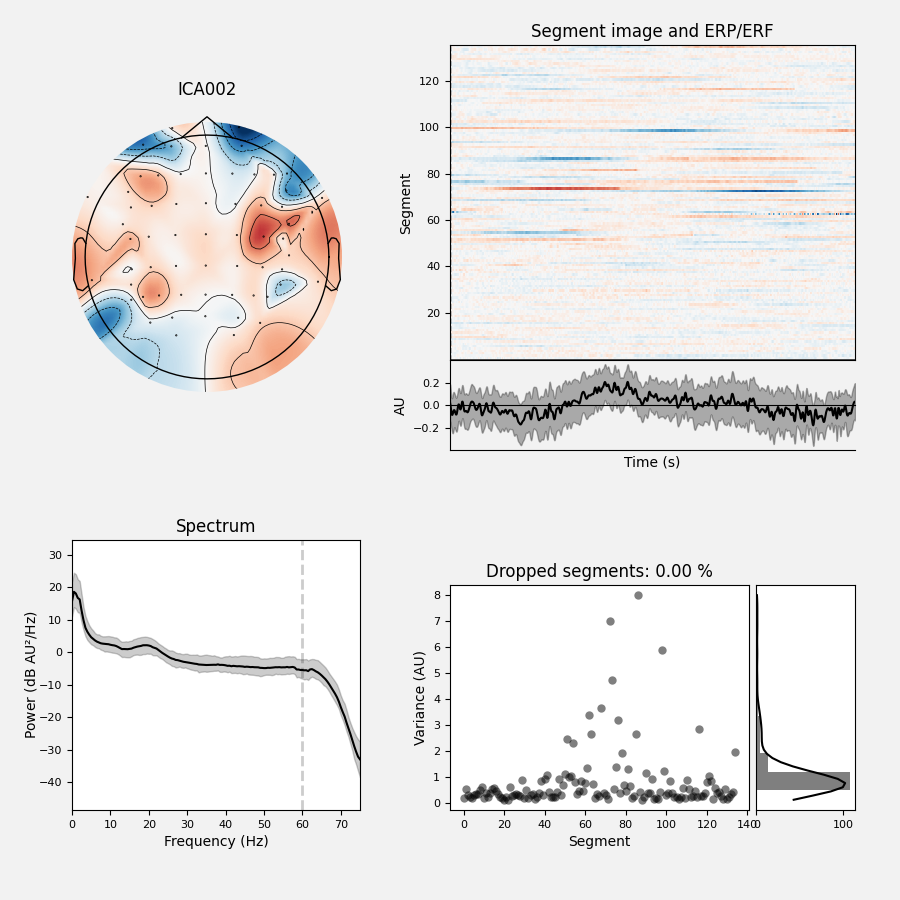
\includegraphics[width=0.8\textwidth]{figs/1_preprocessamento_eeg/4_exemplo_ICA_component_analysis.png}
    \caption{Exemplo de análise detalhada de um componente ICA, apresentando o mapa topográfico, o espectro de frequência e outras características relevantes para a identificação de artefatos.}
    \label{fig:exemplo_ICA_component_analysis}
\end{figure}
\subsection{Pré-processamento do Sinal de ECG}
\label{subsec:preprocess_ecg}

O processamento do sinal de ECG teve como objetivo obter uma versão limpa e refinada, permitindo a detecção precisa dos picos R e a extração de informações de fase. Para isso, os procedimentos foram organizados em três etapas principais: aquisição e segmentação, limpeza do sinal com detecção de picos e aplicação de filtros complementares.

\subsubsection{Aquisição e Segmentação dos Dados de ECG}
\begin{itemize}
    \item \textbf{Aquisição:} Os dados de ECG foram coletados juntamente com informações sobre os tempos de início e fim do período de baseline para cada condição experimental, garantindo a correta identificação dos intervalos de interesse.
    \item \textbf{Segmentação:} Com base nos tempos extraídos dos arquivos de baseline, o sinal bruto foi segmentado para selecionar apenas o intervalo correspondente à condição de interesse. Para reduzir artefatos nas bordas, os primeiros e últimos 15 segundos foram removidos.
\end{itemize}

\subsubsection{Limpeza do Sinal e Detecção de Picos}
\begin{itemize}
    \item \textbf{Limpeza:} Utilizou-se a biblioteca NeuroKit2 para processar o sinal segmentado, removendo ruídos e gerando uma versão limpa do ECG.
    \item \textbf{Detecção Automática de Picos:} Um algoritmo foi aplicado para a detecção automática dos picos R (R-peaks) no sinal limpo, identificando os batimentos cardíacos. A Figura~\ref{fig:ecg_picos_detectados} ilustra um exemplo em que o sinal bruto (cinza) é sobreposto ao sinal limpo (azul), com os picos R destacados em vermelho.
    \item \textbf{Correção Manual dos Picos R:} Após a detecção automática, uma inspeção visual cuidadosa foi realizada utilizando gráficos interativos para:
    \begin{itemize}
        \item Inserir manualmente os picos faltantes, identificados pela ausência de eventos em locais esperados;
        \item Remover manualmente picos falsos, identificados por timestamps incorretos.
    \end{itemize}
    Esse ajuste garante a acurácia na identificação dos batimentos, evitando omissões e inclusões indevidas.
\end{itemize}

\begin{figure}[htb]
    \centering
    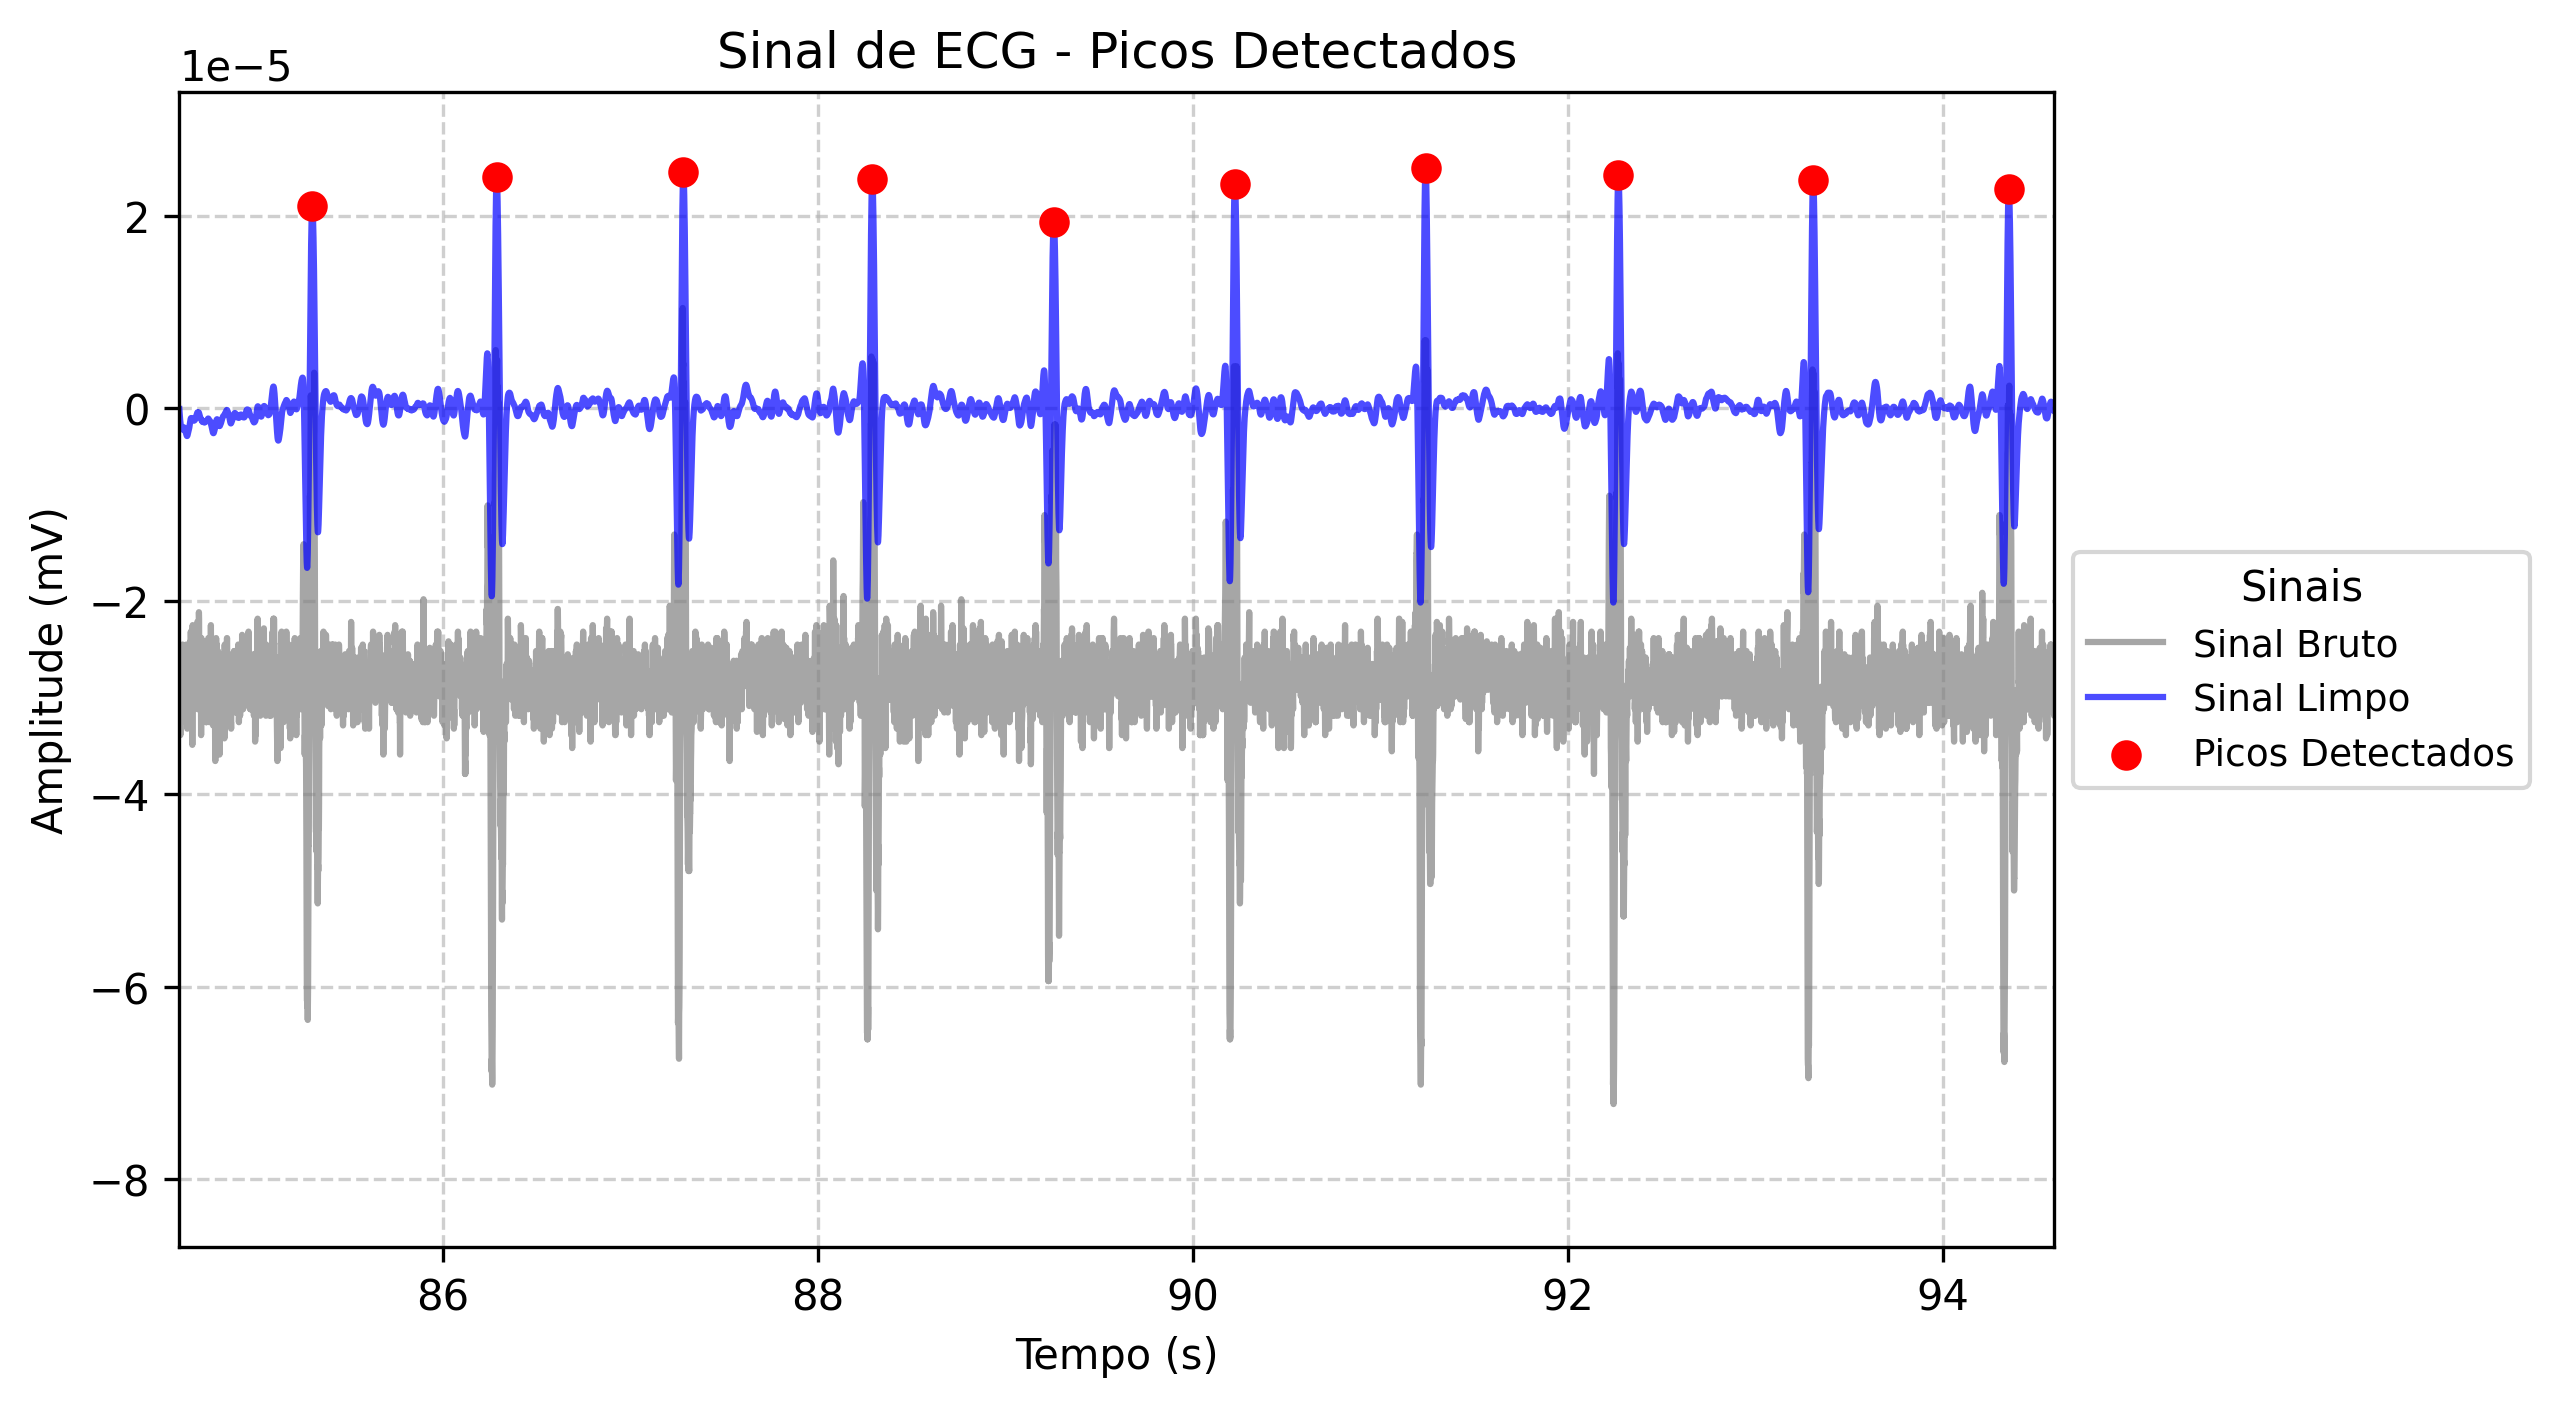
\includegraphics[width=0.8\textwidth]{figs/2_preprocessamento_ecg/1_Sinal_de_ECG_-_Picos_Detectados_zoom.png}
    \caption{Exemplo de sinal de ECG com picos detectados. O sinal bruto (cinza) é sobreposto ao sinal limpo (azul), com os picos R marcados em vermelho.}
    \label{fig:ecg_picos_detectados}
\end{figure}

\subsubsection{Aplicação de Filtros Complementares}
Para refinar a definição dos eventos do ECG, foram aplicados filtros adicionais:
\begin{itemize}
    \item \textbf{Filtro de Janela:} Extração de uma janela de \(\pm50\) ms ao redor de cada pico, isolando os segmentos de interesse.
    \item \textbf{Filtro de Cruzamento pelo Zero:} Identificação dos pontos de cruzamento pelo zero nos segmentos próximos aos picos, permitindo um ajuste fino dos limites dos eventos.
\end{itemize}
A combinação desses filtros resultou em um \emph{Sinal Final Filtrado}, que destaca de forma mais clara a morfologia do ECG. A Figura~\ref{fig:ecg_filtros_aplicados} exemplifica o efeito dos filtros, comparando o sinal limpo inicial (linha colorida) com o sinal final filtrado, bem como os picos detectados.

\begin{figure}[htb]
    \centering
    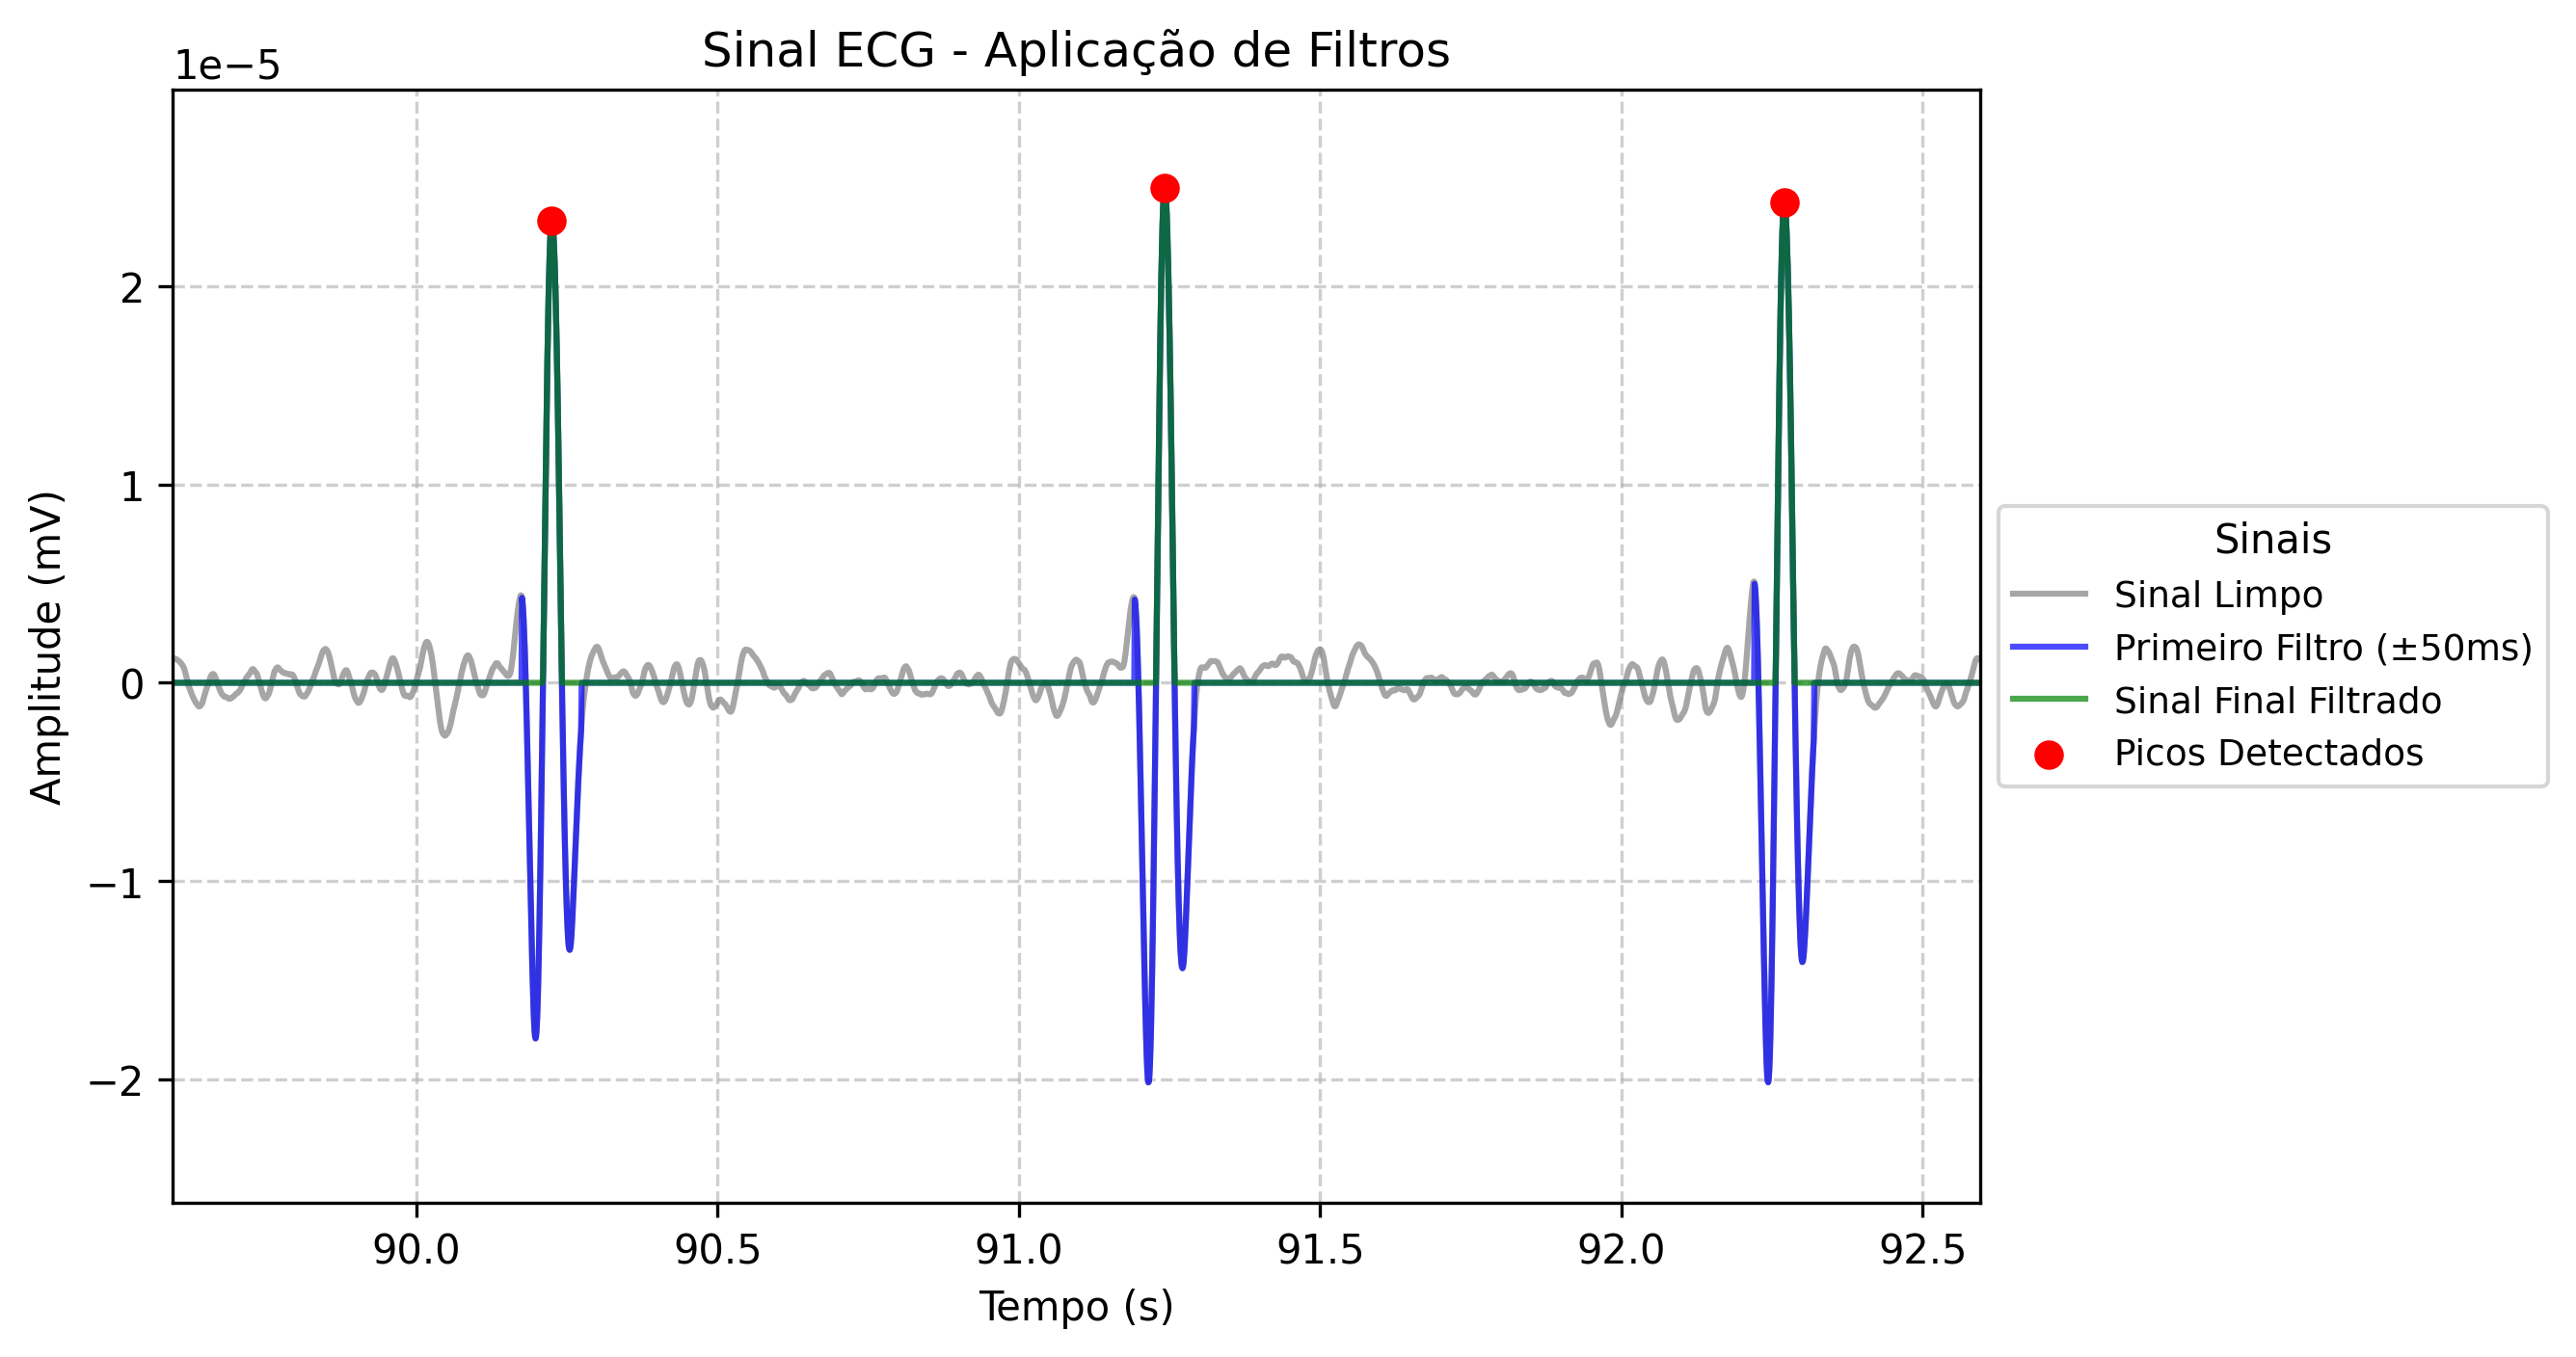
\includegraphics[width=0.8\textwidth]{figs/2_preprocessamento_ecg/2_Sinal_ECG_-_Aplicação_de_Filtros_zoom.png}
    \caption{Exemplo de aplicação de filtros complementares ao sinal de ECG, destacando a morfologia dos picos R (em vermelho).}
    \label{fig:ecg_filtros_aplicados}
\end{figure}
\subsubsection{Geração de Sinais Senoidais e Análise de Fase}

Para aprimorar a análise de sincronização de fase entre os sinais de EEG e ECG, o sinal de ECG foi transformado em uma representação senoidal. Essa transformação apresenta diversos benefícios:
\begin{itemize}
    \item \textbf{Definição Clara do Ciclo Cardíaco:} Ao utilizar os R-peaks para delimitar cada ciclo, a conversão em uma onda senoidal permite definir de forma inequívoca o início e o fim do ciclo cardíaco, fornecendo um marcador preciso para segmentação dos períodos de interesse.
    \item \textbf{Extração Precisa da Fase:} Uma onda senoidal exibe uma variação linear de fase ao longo do tempo, o que facilita a extração da fase instantânea por meio da Transformada de Hilbert, proporcionando uma determinação robusta e consistente.
    \item \textbf{Facilitação da Análise de Sincronização:} Técnicas de sincronização de fase, como o CF-PLM (uma variante do PLV para análise cross-frequency), funcionam melhor quando a fase é clara e bem definida. A representação senoidal torna a fase do ECG mais nítida, permitindo que os algoritmos captem com maior precisão a relação de sincronização entre os ritmos neurais (EEG) e o ritmo cardíaco.
    \item \textbf{Robustez à Variabilidade e Ruído:} A conversão do ECG, que apresenta picos acentuados e variabilidade, para uma forma senoidal suaviza essas irregularidades, melhorando a robustez do método de extração de fase mesmo na presença de ruídos ou artefatos.
    \item \textbf{Integração com a Análise de EEG:} Como os sinais de EEG são frequentemente filtrados para se aproximarem de formas senoidais, padronizar a representação do ECG facilita a integração dos dois tipos de sinal na análise de sincronização, permitindo comparações diretas e métodos cross-frequency mais eficazes.
\end{itemize}

Além desses benefícios, abordagens integradas, como o plugin BrainBeats \cite{cannard2023brainbeats}, facilitam a análise conjunta de sinais de EEG e cardiovasculares, oferecendo ferramentas para a remoção automatizada de artefatos cardíacos e extração de características quantitativas. Estudos como o de Mollakazemi et al. \cite{mollakazemi2021eeg} demonstram que a correta sincronização dos sinais – viabilizada pela transformação do ECG em uma representação senoidal – permite identificar segmentos de EEG com maior relevância funcional, reforçando a importância de uma segmentação temporal precisa na análise de fase.

A Figura~\ref{fig:ecg_comparacao_fase} ilustra a comparação de fase entre o sinal de ECG filtrado (azul), o sinal senoidal gerado (verde) e um sinal simulado (vermelho), evidenciando a coerência de fase entre eles.

\begin{figure}[htb]
    \centering
    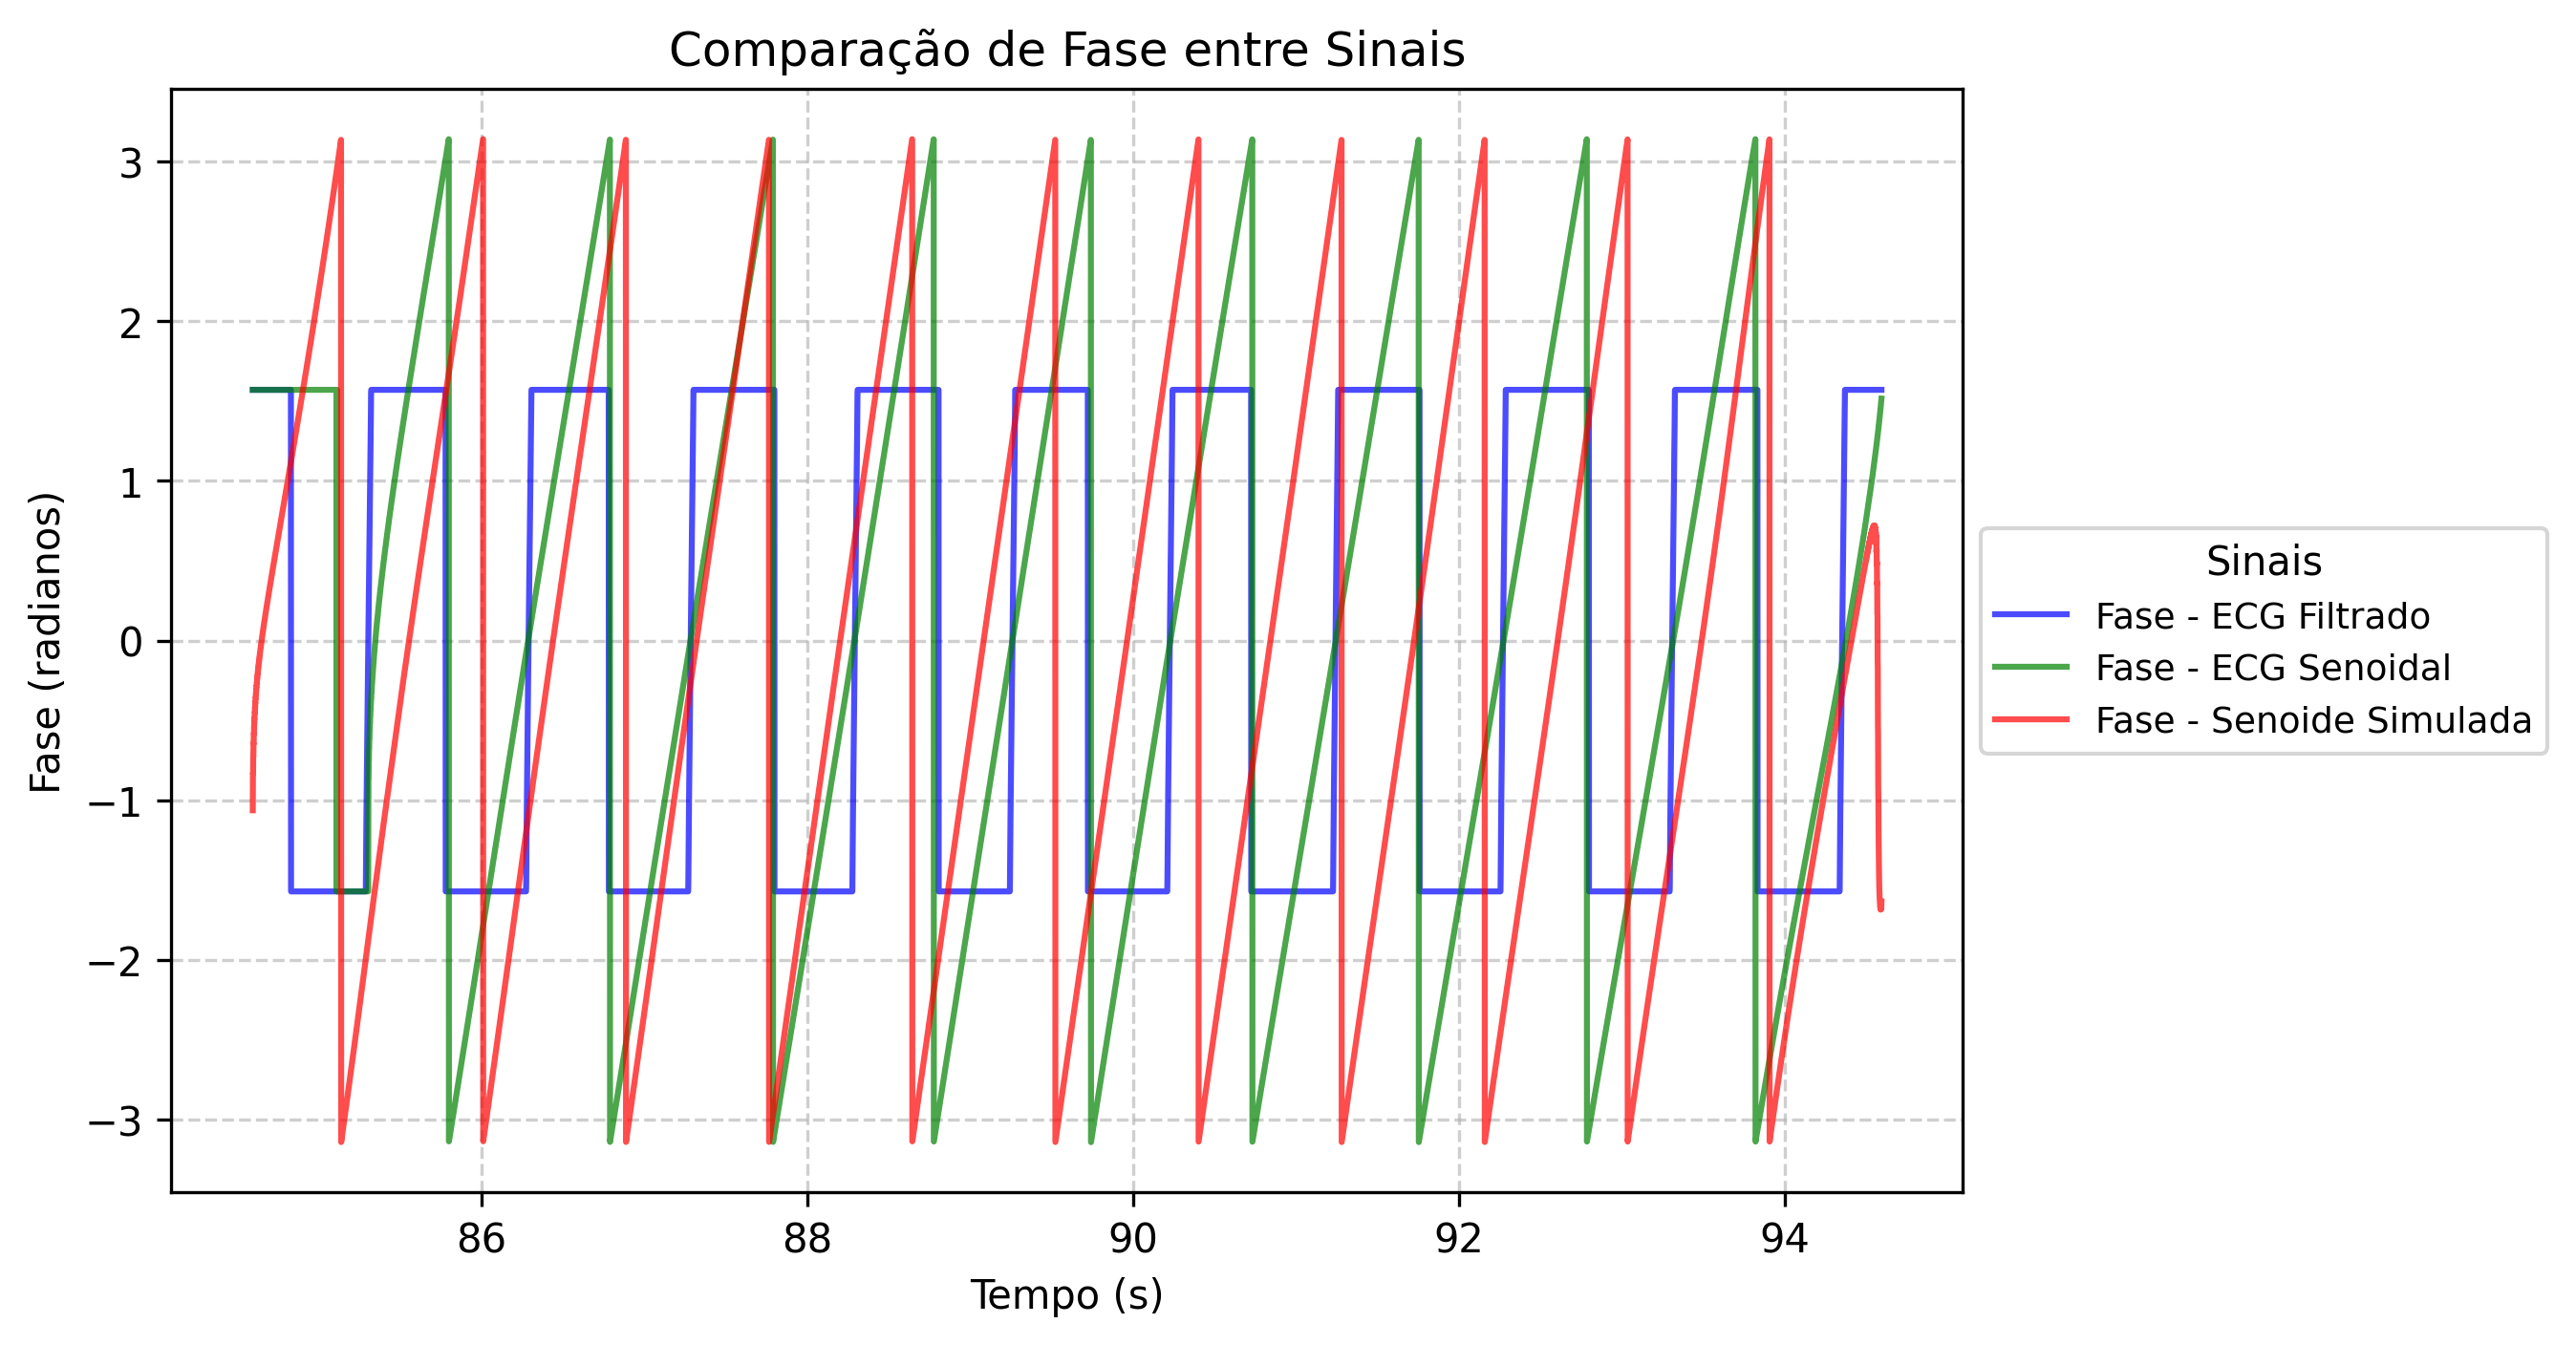
\includegraphics[width=0.8\textwidth]{figs/2_preprocessamento_ecg/3_Comparação_de_Fase_entre_Sinais.png}
    \caption{Exemplo de comparação de fase entre o ECG filtrado (azul), o ECG senoidal (verde) e um sinal simulado (vermelho). A boa concordância entre as fases indica a consistência do procedimento de geração do sinal senoidal e da extração de fase.}
    \label{fig:ecg_comparacao_fase}
\end{figure}

Em suma, a transformação do ECG em um sinal senoidal não apenas define claramente o ciclo cardíaco, mas também possibilita a extração de uma fase contínua, essencial para a análise de sincronização de fase entre EEG e ECG utilizando métodos de extração de fase empregados neste estudo.

\subsubsection{Estrutura do Dado Final e Armazenamento}

O conjunto final de dados resultante do processamento do ECG foi estruturado em um DataFrame que integra as seguintes variáveis:
\begin{itemize}
    \item \textbf{Tempo:} Timestamps sincronizados.
    \item \textbf{Sinal Bruto (EMG):} Valor original do sinal.
    \item \textbf{Sinal Limpo (ECG):} Versão filtrada do sinal.
    \item \textbf{Picos:} Indicador binário dos R-peaks detectados.
    \item \textbf{First Filtered:} Sinal obtido após a aplicação do filtro de janela (\(\pm50\) ms).
    \item \textbf{Final Filtered:} Sinal final obtido após a combinação dos filtros aplicados.
    \item \textbf{ECG Senoidal:} Sinal senoidal derivado dos R-peaks.
\end{itemize}

Este DataFrame foi exportado em formato CSV para facilitar o acesso e a análise subsequente dos dados.
